\documentclass{article}
\usepackage{geometry}
\usepackage{flafter}
\geometry{letterpaper, portrait, margin=1in}
\usepackage{hyperref}
\hypersetup{
    colorlinks=true,
    linkcolor=black,
    filecolor=magenta,
    urlcolor=blue,
}
\usepackage{graphicx}
\graphicspath{ {images/} }

\usepackage{tcolorbox}
\usepackage{textcomp}
\usepackage{gensymb}
\usepackage{indentfirst}
\newcommand{\ans}{$\rule{1.5cm}{0.15mm}$}

\newcommand{\icon}[1]{\includegraphics[height=2.75\fontcharht\font`\B]{#1}}

\title{EAGLE Cheat Sheet}
\author{Asha Bhandarkar}
\date{July 2019}

\begin{document}
\maketitle{}
\setcounter{tocdepth}{3}

\pagebreak

\section{Schematic Window}
\begin{figure}[ht]
	\center
	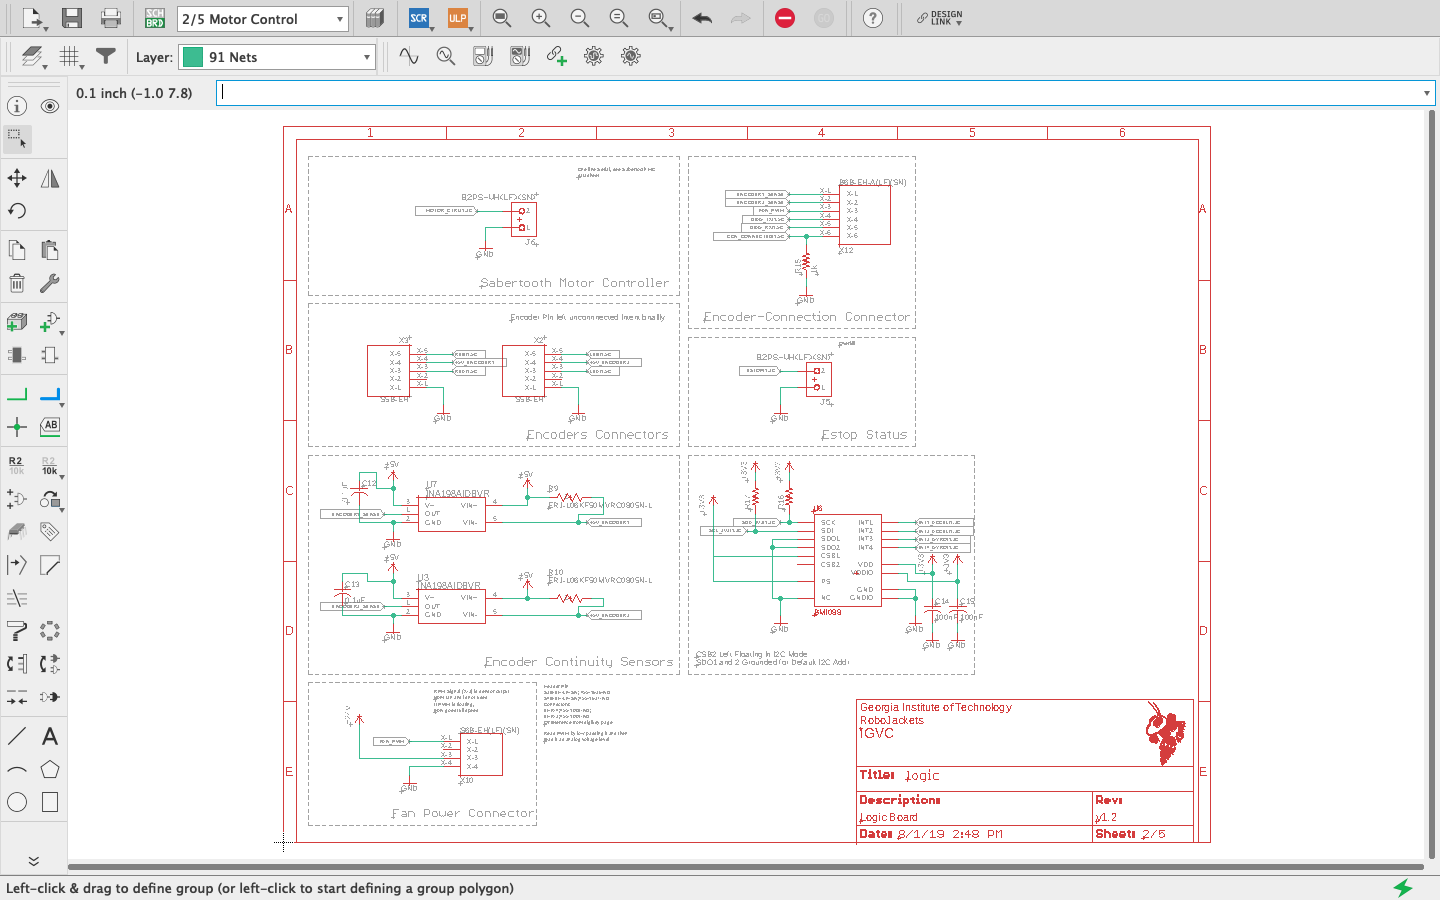
\includegraphics[width=\textwidth, keepaspectratio]{mainschematic.png}
	\caption{An example of what the schematic window looks like in EAGLE. This is the motor control sheet for IGVC's Logic Board v1.2.}
	\label{fig:schematic window}
\end{figure}


\subsection{Libraries}
\subsubsection{Adding Libraries}
\begin{itemize}
    \item Open the Library Manager using the \icon{libraryman.png} icon to add libraries that contain the parts you will need in your design.
\end{itemize}


\subsection{Parts}
\subsubsection{Adding Parts}
\begin{itemize}
    \item Open the Add window using the \icon{partadd.png} icon or using the \texttt{add} command to see available libraries to add parts from.
\end{itemize}
\subsubsection{Viewing Properties}
\begin{itemize}
    \item Open using the \icon{info.png} icon or using the \texttt{info} command.
    \begin{itemize}
        \item You can change various properties such as Name, Position, and Angle.
        \item You can see the Device, Footprint, and Library of the part.
    \end{itemize}
\end{itemize}
\subsubsection{Positioning}
\begin{itemize}
    \item Use the \icon{move.png} icon or the \texttt{move} command to move parts.
    \item Use the \icon{mirror.png} icon or the \texttt{mirror} command + left-click to mirror parts.
    \item Use the \icon{rotate.png} icon or the \texttt{rotate} command + left-click to rotate parts.
\end{itemize}
Note: Many of these commands plus more can be accessed by right-clicking the part.

\subsection{Connections}
\subsubsection{Drawing Nets}
\begin{itemize}
    \item Use the \icon{net.png} icon or the \texttt{net} command to draw electrical connections between parts.
\end{itemize}
\subsubsection{Adding Junctions}
\begin{itemize}
    \item Use the \icon{junction.png} icon or the \texttt{junction} command to indicate a shared electrical connection.
\end{itemize}
\subsubsection{Adding Labels}
\begin{itemize}
    \item Use the \icon{label.png} icon or the \texttt{label} command to create breakouts for more complex schematics. These labels display the Name property of the net.
    \begin{itemize}
        \item Use the top bar to select the XREF label format.
    \end{itemize}
\end{itemize}

\subsection{Organization}
\subsubsection{Managing Sheets}
\begin{itemize}
    \item Use the \icon{sheet.png} dropdown to add, remove, and toggle between sheets in a schematic. 
\end{itemize}
\subsubsection{Layers}
\begin{itemize}
    \item Use the \icon{schlayer.png} dropdown to toggle between layers in the schematic.
\end{itemize}

\subsection{Review}
\subsubsection{Running ERC}
\begin{itemize}
    \item Use the \icon{erc.png} icon or the \texttt{erc} command to run error checking on your schematic.
\end{itemize}
\subsubsection{Switching to Board Layout}
\begin{itemize}
    \item Use the \icon{schbrd.png} icon to open the board layout window from the schematic window.
\end{itemize}

\pagebreak

\section{Board Layout}
\begin{figure}[ht]
	\center
	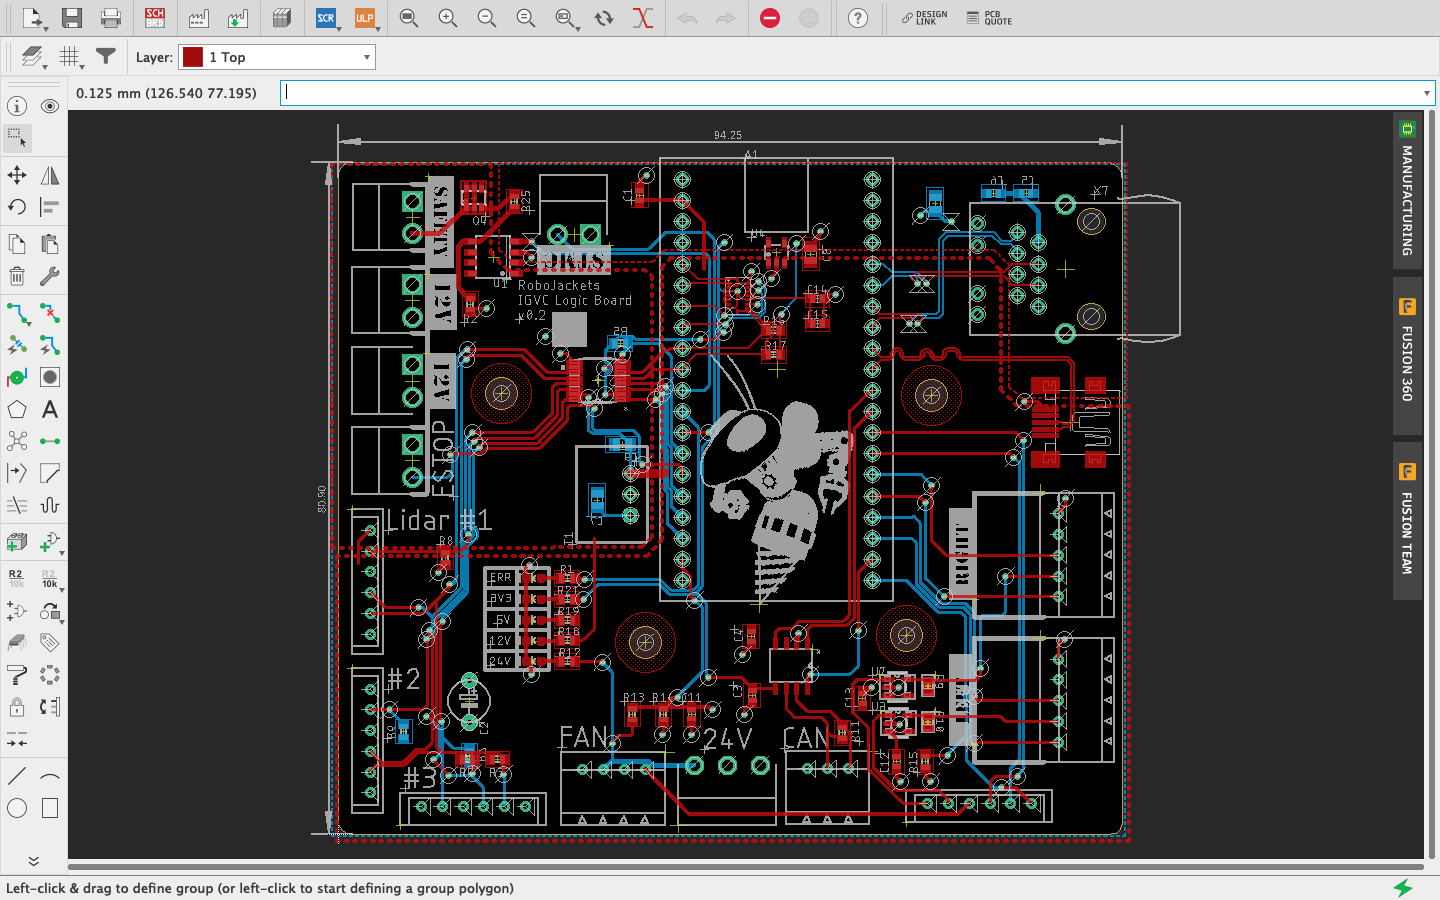
\includegraphics[width=\textwidth, keepaspectratio]{boardlayout.png}
	\caption{An example of what the board layout window looks like in EAGLE. This is IGVC's Logic Board v1.2.}
	\label{fig:board layout window}
\end{figure}


\subsection{Parts}
\subsubsection{Viewing Properties}
\begin{itemize}
    \item See section 1.2.2
\end{itemize}

\subsubsection{Positioning}
\begin{itemize}
    \item Use the \icon{ratsnest.png} icon or the \texttt{ratsnest} command to readjust airwires (lines that represent electrical connections on the PCB layout) and fill in polygons.
    \item See section 1.2.3 
\end{itemize}

\subsection{Connections}
\subsubsection{Adding Traces}
\begin{itemize}
    \item Use the \icon{route.png} icon or the \texttt{route} command to connect airwires. 
    \begin{itemize}
        \item Dropdown on icon gives options to route multiple signals, a differential pair, etc. 
        \item Top bar gives options to change trace width, obstacle avoidance, trace angle (right-click shortcut), etc. 
        \item EAGLE does have an autorouter. You \textbf{should not} use this to route your boards. 
    \end{itemize}
\end{itemize}
\subsubsection{Deleting Traces}
\begin{itemize}
    \item Use the \icon{ripup.png} icon or the \texttt{ripup} command to undo traces.
    \begin{itemize}
        \item Use the \texttt{ripup;} command to undo all traces.
        \item Use the backspace key to delete segments while routing.
    \end{itemize}
    \item Use the \texttt{ripup <POLYGON NAME>} command to delete polygons.
    \begin{itemize}
        \item Use the \texttt{ripup @ < POLYGON NAME>} command to unfill polygons and \texttt{ripup @;} to unfill all polygons.
    \end{itemize}
\end{itemize}
\subsubsection{Adding Vias}
\begin{itemize}
    \item Use the \icon{via.png} icon or the \texttt{via} command to place connections between layers.
    \begin{itemize}
        \item Top bar gives option to change drill size (Note that what DRC you use might limit the changes you can make).
        \item Use the space bar to add vias while routing.
    \end{itemize}
\end{itemize}
\subsubsection{Drawing Polygons}
\begin{itemize}
    \item Use the \icon{polygon.png} icon or the \texttt{polygon} command to draw planes.
    \begin{itemize}
        \item Thermal pads can be turned off (turned on by default) in the top bar.
    \end{itemize}
\end{itemize}

\subsection{Organization}
\subsubsection{Layers}
\begin{itemize}
    \item Use the \icon{brdlayer.png} dropdown to toggle between layers on the PCB.
    \begin{itemize}
        \item Use the spacebar to toggle between layers to select the layer you want to route on.
        \item Use \icon{layersettings.png} icon to access layer settings and create preset layers.
    \end{itemize}
\end{itemize}

\subsection{Review}
\subsubsection{Running DRC}
\begin{itemize}
    \item Use the \icon{drc.png} or the \texttt{drc} command to run error checking on your board layout.
    \item In the DRC pop up window you can load specific DRCs to run.
\end{itemize}
\subsubsection{Switching to Schematic Window}
\begin{itemize}
    \item Use the \icon{brdsch.png} icon to open the schematic window from the board layout window.
\end{itemize}







\end{document}

